\documentclass[a4paper,12pt]{article} 
\usepackage[T1]{fontenc}              
\usepackage[frenchb]{babel} % césures, titres français
\usepackage[utf8]{inputenc} % encodage
\usepackage[a4paper,left=3cm,right=3cm,top=2cm,bottom=2cm]{geometry} % marges
\usepackage{graphicx} % insertion d'images
\usepackage{rotating}
\usepackage{float} % permet d'utiliser H pour placer un flottant obligatoirement
\usepackage{pdfpages} % inclusion de PDF au sein du document
\usepackage{listings}
\pagestyle{plain} % pied de pages simples

\setlength{\parskip}{1ex plus 0.5ex minus 0.2ex} % espace entre les paragraphes
\setcounter{tocdepth}{2}
\setcounter{secnumdepth}{2}

\lstset{% general command to set parameter(s)
basicstyle=\ttfamily, % print whole listing small
keywordstyle=\color{black}\bfseries\underbar,
% underlined bold black keywords
identifierstyle=, % nothing happens
commentstyle=\color{white}, % white comments
showstringspaces=false,
numbers=left,
language=java,
breaklines=true,
frame=tblr} % no special string spaces

%%%% debut macro %%%%
\makeatletter
\renewcommand\section{\@startsection {section}{1}{\z@}%
                           {-3.5ex \@plus -1ex \@minus -.2ex}%
                           {2.3ex \@plus.2ex}%
                           {\normalfont\Large\bfseries}}
\makeatother
%%%% fin macro %%%%



% Def
\newcommand{\code}[1]{{\lstinline{#1}}}

\begin{document}
\newpage
\title{TP Sécurité des réseaux}
\author{BRIZAI Olivier\\THORAVAL Maxime}
\maketitle

\newpage
\tableofcontents
\newpage


\section{Introduction}
Le but de ce TP est de mettre en place un réseau sécurisé à l'aide d'un firewall CISCO ASA.\\
Ci-dessous, le réseau que nous souhaitons obtenir (les règles de filtrage ne sont pas représentées).

\begin{figure}[H]
	\center
	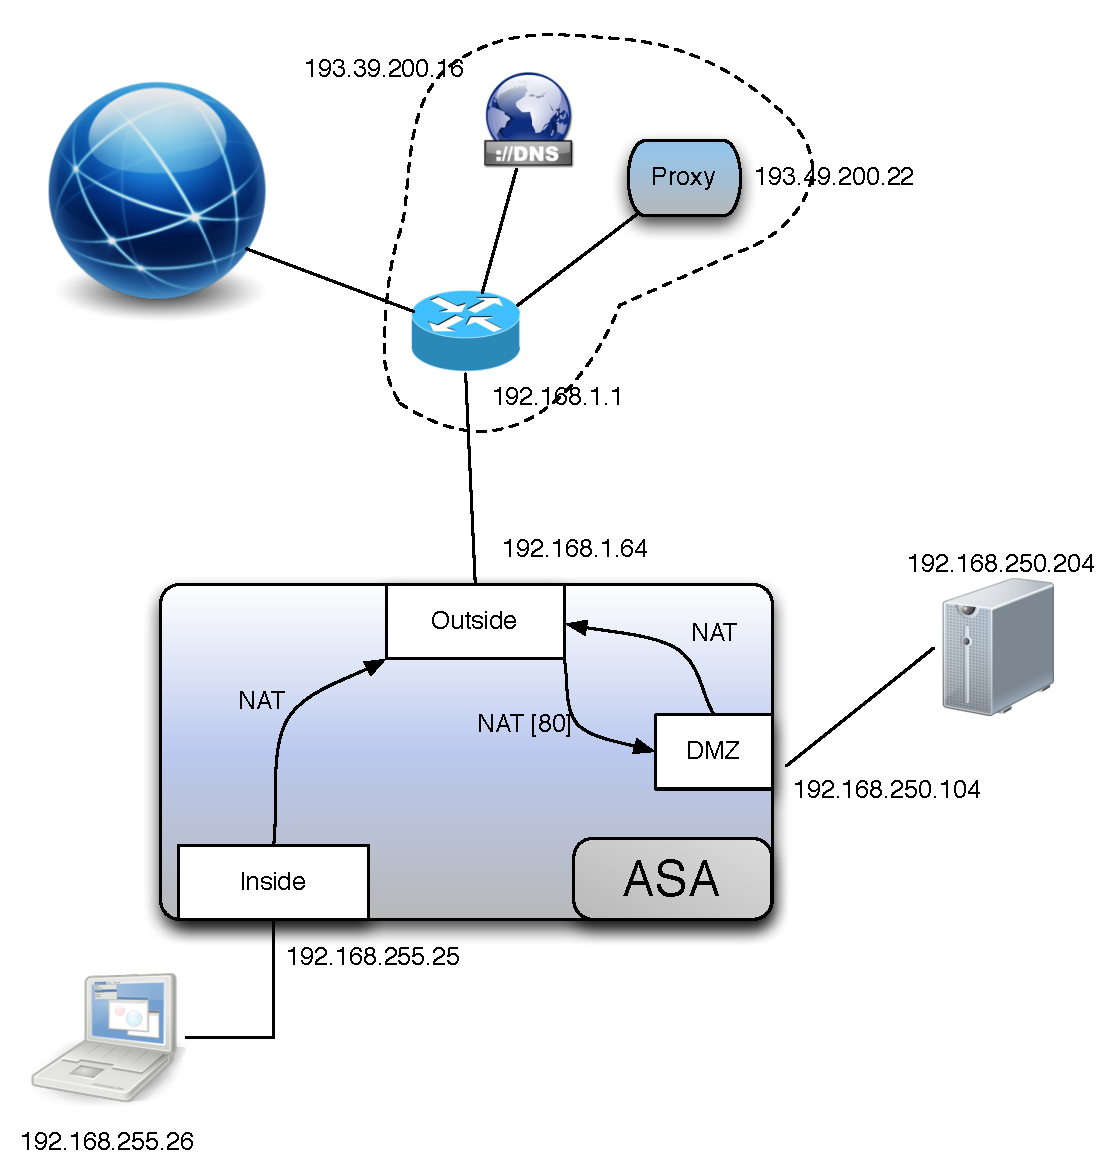
\includegraphics[width=15cm]{img/reseau.pdf}
	\caption{Réseau à obtenir}
\end{figure}

\newpage




\section{Installation}

Dans un premier temps, nous avons installé Ubuntu 9.04 (version client) sur notre PC. Celle-ci effectuée, nous réalisons les démarches suivantes, c'est à dire mise en place de Java ainsi que l'installation du paquet \og Minicom \fg.

Nous lançons ensuite la commande \textbf{minicom -s} et définissons les divers paramètres afin de configurer le port console. Puis, nous définissons l'adresse \textit{inside} de l'ASA. Nous pouvons maintenant, à partir de celle-ci, accéder à l'interface d'administration de l'ASA au sein de notre navigateur.\\La figure ci-dessous présente l'accueil de celle-ci. 

\begin{figure}[H]
	\center
	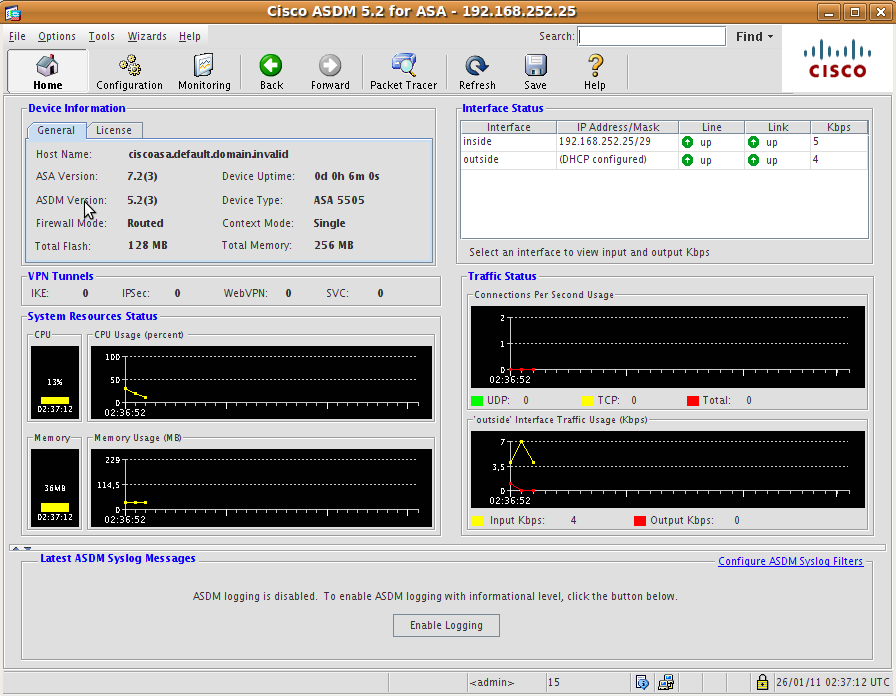
\includegraphics[width=15cm]{img/1-Interfaceconfigfw.png}
	\caption{Interface de configuration}
\end{figure}

Nous avons ensuite utilisé le \og Wizard \fg de l'application pour mettre en place un certain nombres de paramètres tel que adresses IP (inside, outside, dmz) ou encore la répartition des interfaces du firewall (cf. figure ci-dessous). 
\begin{figure}[H]
	\center
	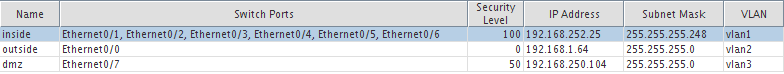
\includegraphics[width=15cm]{img/2-Interfaces.png}
	\caption{Configuration des interfaces}
\end{figure}





\section{Configuration Inside}
Dans cette partie, nous avons configuré notre firewall afin de permettre certaines actions à l'interface \textit{inside}.

\subsection{Configuration du NAT}
Dans un premier temps, il nous a fallu configurer une règle de NAT afin de traduire l'adresse privée de l'interface \textit{inside} en l'adresse publique de l'interface \textit{outside}. Nous devons effectuer cette étape car il a été défini que les adresses privé (type 192.168.x.x) ne sont pas visibles sur internet. Ceci est dû au fait que nous arrivons à pénurie des adresse IPv4.\\
Ci-dessous, la configuration de notre NAT, pour le sous-réseau de lié à notre interface \textit{inside} (192.168.252.24), nous lions l'adresse de l'interface \textit{outside}.
\begin{figure}[H]
	\center
	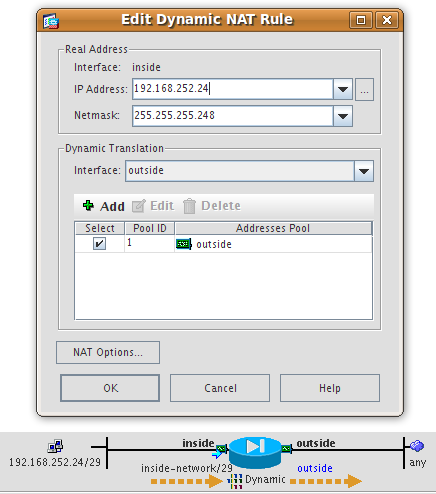
\includegraphics[width=13cm]{img/3-ConfigurationduNAT.png}
	\caption{Configuration du NAT}
\end{figure}


\subsection{Règles de filtrage}
Notre NAT crée, nous allons maintenant mettre en place des règles de filtrage afin de ne laisser passer que les paquets liés à des servies définis.

Dans un premier temps, nous autorisations les flux TCP et UDP sur le port 53 (DOMAIN) qui sont à destination de 193.49.200.16 (adresse du serveur DNS de l'ENSICAEN).\\
Ci-dessous ces deux règles.
\begin{figure}[H]
	\center
	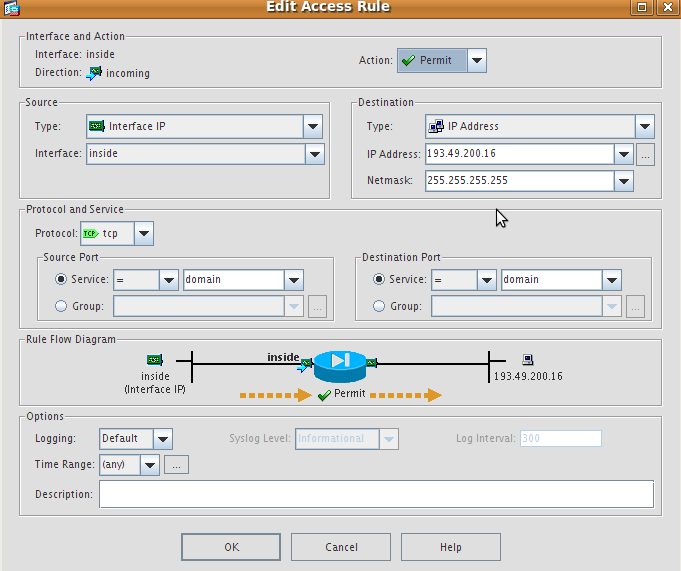
\includegraphics[width=15cm]{img/4-RegleTCP(DOMAIN).png}
	\caption{Règle 1 : TCP DOMAIN}
\end{figure}
\begin{figure}[H]
	\center
	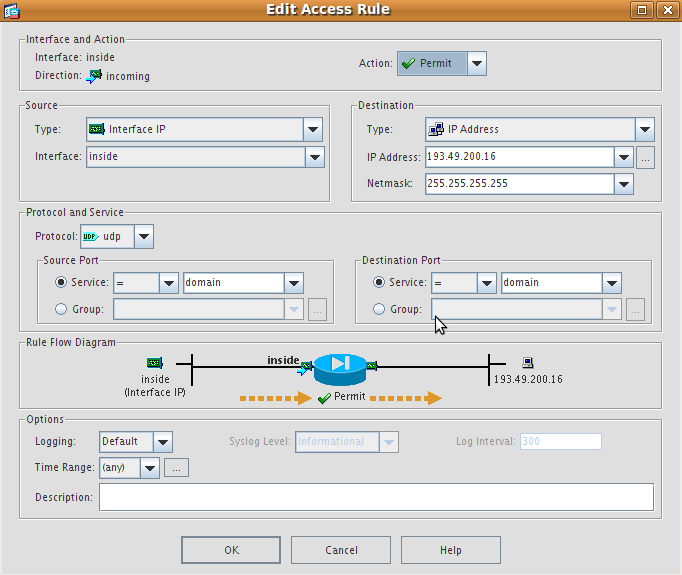
\includegraphics[width=15cm]{img/4-RegleUDP(DOMAIN).png}
	\caption{Règle 1 : UDP DOMAIN}
\end{figure}


\newpage
Maintenant, nous créons la règle autorisant le flux SSH (TCP sur le port 22) qu'importe le destinataire.
\begin{figure}[H]
	\center
	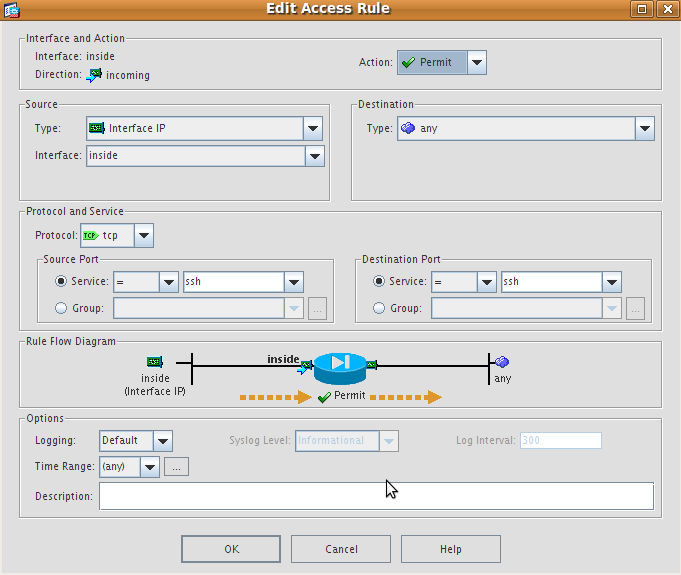
\includegraphics[width=15cm]{img/5-RegleSSH.png}
	\caption{Règle 2 : SSH}
\end{figure}


\newpage
Puis la règle autorisant le flux HTTP (TCP sur le port 80) à destination de 193.49.200.22 (adresse du proxy de l'ENSICAEN).
\begin{figure}[H]
	\center
	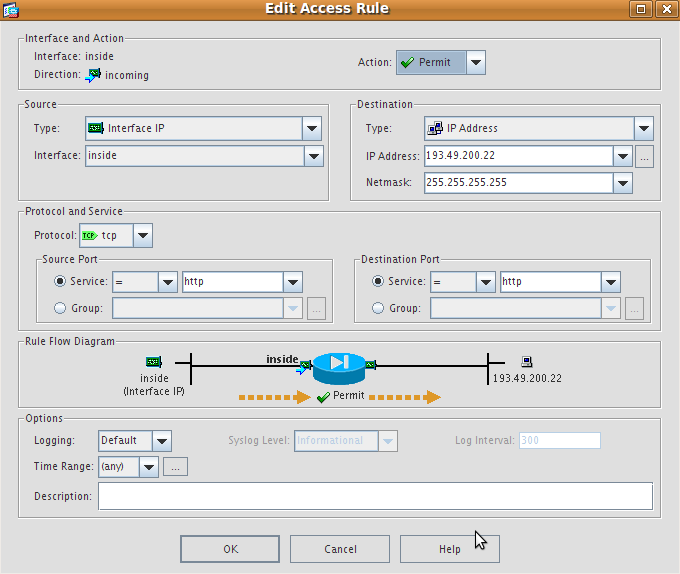
\includegraphics[width=15cm]{img/6-RegleHTTP.png}
	\caption{Règle 3 : HTTP}
\end{figure}


\newpage
Enfin, nous autorisons le flux à destination d'un proxy (TCP sur le port 3128 = port du proxy de l'école). Bien entendu, nous nous restreignons une nouvelles fois à l'adresse du proxy de l'ENSICAEN. 
\begin{figure}[H]
	\center
	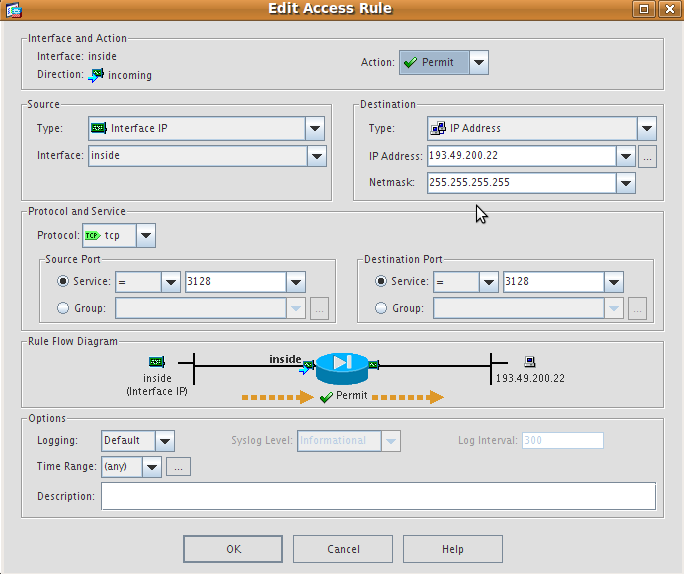
\includegraphics[width=15cm]{img/7-RegleProxy.png}
	\caption{Règle 4 : Proxy}
\end{figure}


\newpage
Nous sommes maintenant censé pouvoir accéder au routeur de l'école (adresse 192.168.1.1). Pour le vérifier, nous lançons la commande \textbf{ping} sur son adresse. On remarque que nous n'avons pas de retour de cette commande. Afin de vérifier l'erreur, nous allons regarder le \textit{monitoring} de notre firewall. Ceci va nous permettre de suivre son activité. Après analyse des traces, nous avons pu comprendre l'échec de la commande \textbf{ping}. En effet, elles nous informent que les paquets de type ICMP ne sont pas autorisés à destination de l'interface \textit{inside}. Afin de résoudre ce problème, nous devons rajouter une nouvelle règle de filtrage que nous avons défini de la manière ci-dessous.
\begin{figure}[H]
	\center
	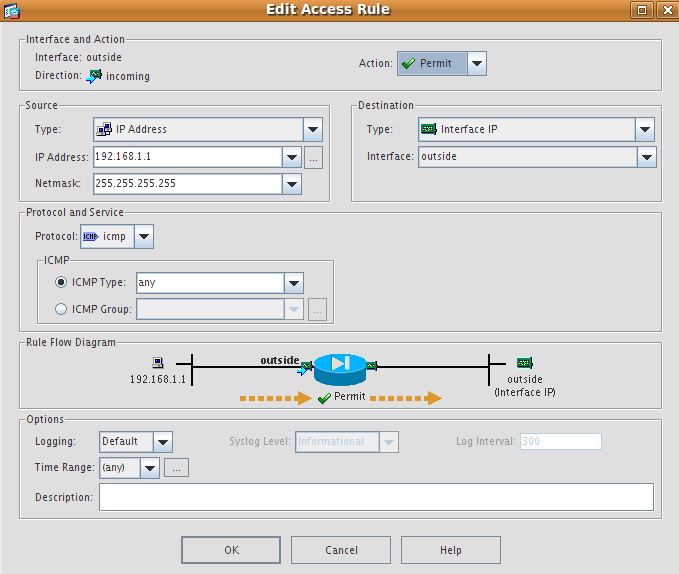
\includegraphics[width=13cm]{img/8-Pingrevientpasflitrageicmp.png}
	\caption{Filtrage ICMP pour autoriser le retour de ping}
\end{figure}

Cette règle mise en place, nous lançons une nouvelles fois la commande \textbf{ping}. Comme visible sur la figure ci-dessous, il n'y a plus d'échec.
\begin{figure}[H]
	\center
	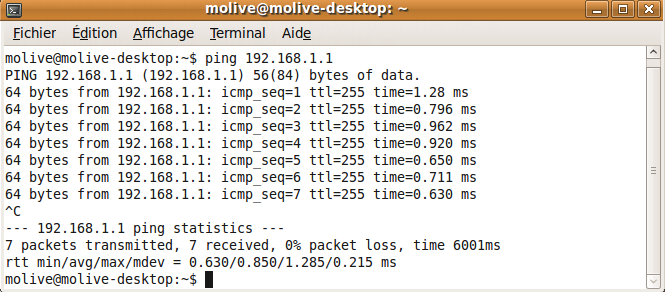
\includegraphics[width=13cm]{img/9-pingok.png}
	\caption{Résultat ping}
\end{figure}




\section{Configuration DMZ}
\subsection{Installation}
Nous souhaitons maintenant configurer la DMZ. Dans un premier temps, nous installons \og Ubuntu 9.0.4 server \fg{} sur le PC relié à l'interface DMZ du firewall. Lors de l'installation, nous indiquons que nous souhaitons avoir par défaut les services suivants : un serveur SSH et un serveur web (LAMP).

L'installation terminée, nous allons maintenant configurer les informations réseau de notre serveur. Nous renseignons son adresse IP (192.168.250.204), le masque associé et enfin le routeur (ici il s'agit de l'adresse de l'interface \textit{dmz} de notre firewall).\\
Afin de mettre en place ces informations, nous allons modifier le fichier \textit{/etc/network/interfaces} de la sorte :
\begin{lstlisting}
auto eth0 
iface eth0 inet static
    address 192.168.250.204
    netmask 255.255.255.0
    gateway 192.168.250.104
\end{lstlisting}

\newpage
\subsection{Règles de filtrage}
Comme pour notre interface \textit{inside}, nous allons devoir indiquer un certain nombre de règles de filtrage pour autoriser différents service.

Dans un premier temps, nous souhaitons que toutes les requêtes HTTP provenant de l'interface \textit{inside} à destination de la \textit{dmz} puissent être transmises. Ci-dessous, la règle liée. 
\begin{figure}[H]
	\center
	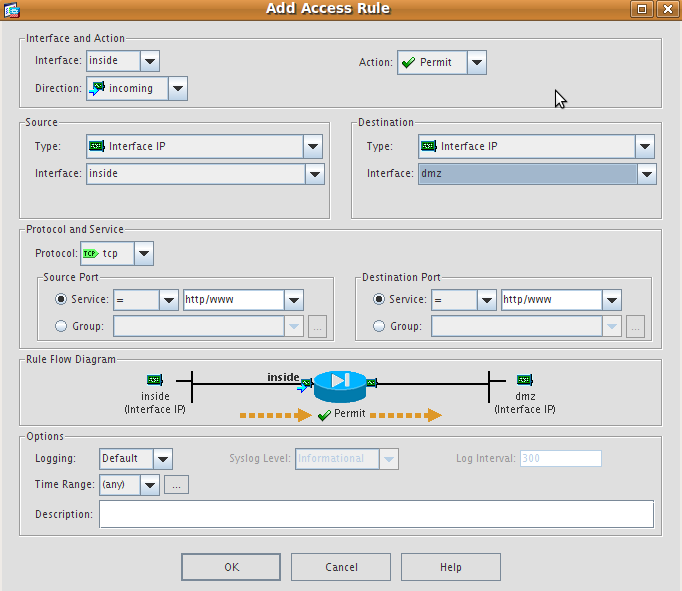
\includegraphics[width=15cm]{img/10-httpinsidedmz.png}
	\caption{Règle 1 : HTTP inside vers dmz}
\end{figure}

\newpage
Nous souhaitons aussi que les requêtes HTTP externes puissent être reçu par la \textit{dmz}, dans ce cas, nous devons définir une nouvelle règle autorisant ces flux entre l'interface \textit{outside} et la \textit{dmz}.
\begin{figure}[H]
	\center
	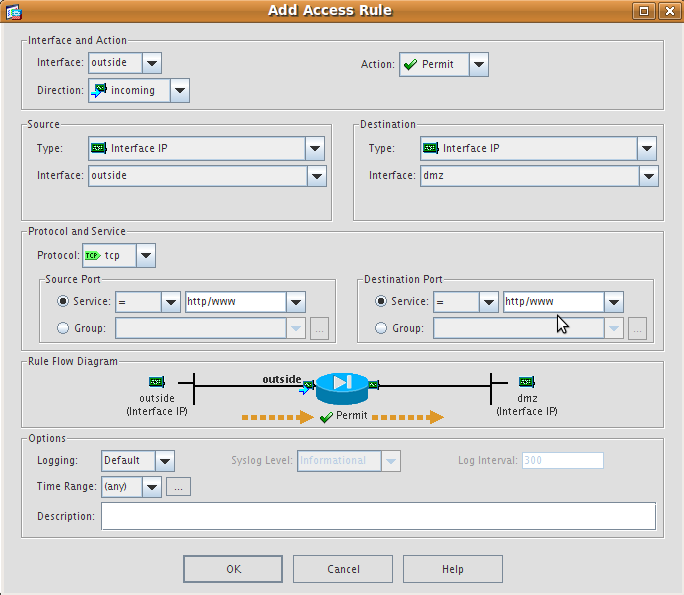
\includegraphics[width=15cm]{img/11-httpoutsidedmz.png}
	\caption{Règle 1 : HTTP outside vers dmz}
\end{figure}

\newpage
Enfin, nous faisons de même pour les requêtes SSH.
\begin{figure}[H]
	\center
	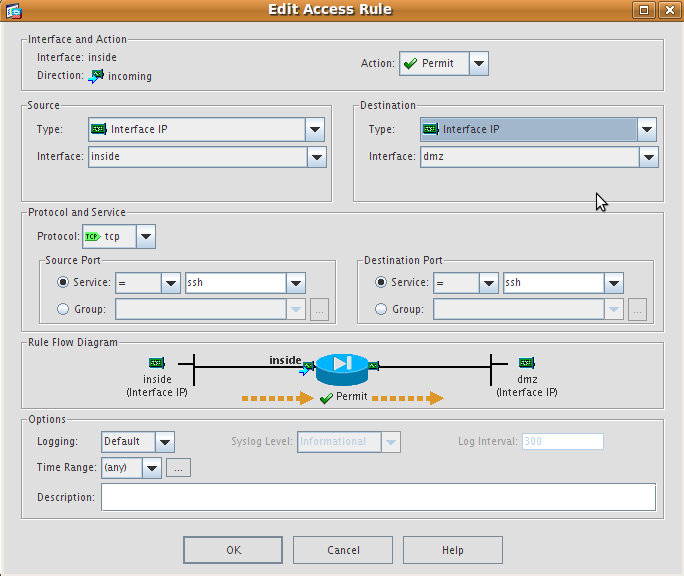
\includegraphics[width=12cm]{img/12-sshinsidesmz.png}
	\caption{Règle 2 : SSH inside vers dmz}
\end{figure}
\begin{figure}[H]
	\center
	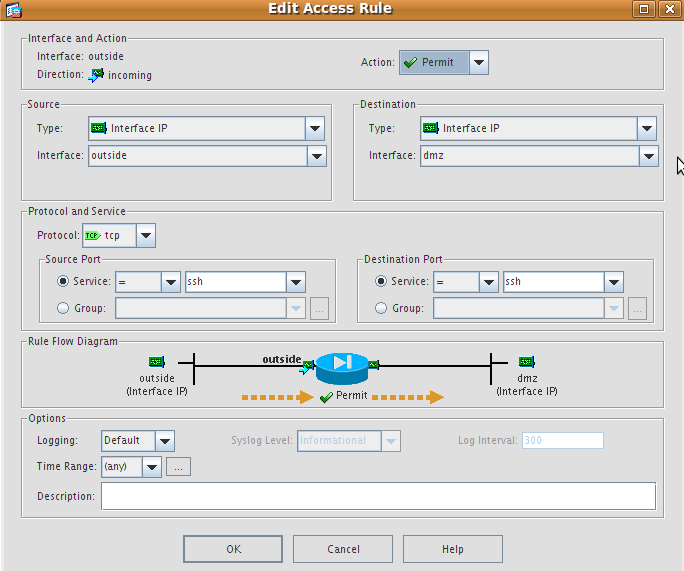
\includegraphics[width=12cm]{img/13-sshoutsidedmz.png}
	\caption{Règle 2 : SSH outside vers dmz}
\end{figure}

\end{document}




